%%% writeup.tex --- 

%% Author: bh0085@Ben13.local
%% Version: $Id: proposal.tex,v 0.0 2010/11/21 05:40:38 bh0085 Exp$


\documentclass[12pt,a4paper]{article}
\usepackage[hmargin=1in,vmargin=1in]{geometry}
\usepackage{natbib}
\usepackage{amsmath}
\usepackage{amssymb} % allow blackboard bold (aka N,R,Q sets)

%%\usepackage{times}
\usepackage[debugshow,final]{graphicx}

%%\revision$Header: /Users/bh0085/Documents/Fellowship/NSF/proposal/proposal.tex,v 0.0 2010/11/21 05:40:38 bh0085 Exp$

\begin{document} 
\setlength{\parindent}{5ex} 
\setlength{\parskip}{0ex}
\renewcommand{\thefootnote}{\alph{footnote}}
\noindent\textbf{Phylogenetic tests for conservation of multiple structures in ncRNA families} 
\noindent Ben Holmes
\section{Abstract}
Phylogenetic databases of functional, non-coding RNAs (ncRNAs) such as Rfam\footnote{http://rfam.sanger.ac.uk/} sort sequences into families according to homology to single structural profiles. Supposing that some of the myriad alternative foldings of these families will be present in vivo and seeing no prior reason to rule out the biological importance of RNAs in alternative conformations, this paper attempts a systematic investigation of the likelihood that evolution acts to conserve structural alternates in $\approx$1000 such Rfam families. By a combination of thermodynamic and phylogenetic methods using novel and published algorithms, I observe several families where natural selection appears to be acting to preserve alternative foldings over Rfam families and suggest improvements to my method that could yield many more.


\section{Background}
One major product of ongoing efforts to re-evaluate the central dogma of molecular biology is available to biologists in the form of huge databases of untranslated RNAs (ncRNAs) such as Rfam. Grouped into families sharing similar secondary (and presumably tertiary) structures, conserved ncRNAs have been demonstrated to play roles in a wide variety of processes in all domains of life. 

As transcriptomics have yielded functional roles for these ncRNAs, structural biologists have worked to associate form with function. Here, techniques from protein structure determination such as x-ray crystallography (XRC) and NMR have been applied with mixed success. The former provides fine structure resolution but necessitates growth of RNA crystals that are difficult to obtain for many ncRNAs. The latter is carried out in vitro but gives lower resolution structures and works only for small relatively short sequences.

Meanwhile, computational methods to efficiently identify stable RNA foldings have been around for decades. Because a large fraction of the energy change of RNA folding is accounted for in 2D secondary structure, efficient algorithms can compute thermodynamically optimal and suboptimal \cite{RefWorks:17} foldings. Modern thermodynamic techniques such as RNAfold \cite{RefWorks:24} compute foldings using a number of experimentally derived parameters while another set of techniques such as EvoFold \cite{RefWorks:21} implement stochastic context free grammars (SCFGs) to predict foldings from evolutionary signatures.

For some ncRNAs, thermodynamic and SCFG methods enjoy strong agreement with physical methods and one another. In others, thermodynamic methods suggest that ncRNAs can fold to a number of suboptimal shapes whereas our understanding of their function may be based on a single structure obtained by NMR or XRC. While previous works \cite{RefWorks:22} have designed prediction methods incorporating thermodynamic and evolutionary models, the two approaches often fail for the same structures. 

Thus, outside of the relatively small subset of ncRNAs for which the specific role of folded structure in enabling biological activity have been deduced by detailed biochemical investigation\footnote{and for which reaction mechanisms analogous to peptide based enzymes have been characterized}, the specific role of structure in ncRNA function is largely mysterious. In so far as databases such as Rfam group these RNAs by homology to single structural profiles - deduced for example by hidden markov models (HMMs)\footnote{http://infernal.janelia.org/}, ncRNAs are named and classified under the implicit assumption that their biological activity is dependent upon folding to a single structure. In this light, alternative conformations are labelled ``suboptimal'' as much for their presumably degraded biological activity as their (often minimally) reduced negative free energies of folding.

The majority of traditional folding algorithms therefore strive to pinpoint optimal structures by incorporating additional information or iteratively constructing alignments refined by best folding solutions found in previous steps. As better foldings reduce structural entropy, the alignments that they imply will correspondingly refine and final solutions are bound to reflect single optima with enhanced clarity. 

Thus while naive energy models predict that ncRNAs may fold to various secondary structures at negative thermodynamic potentials, most descriptions of RNA families are phrased in terms of single consensus structures and are graded largely by the extent to which they do so. To the extent that thermodynamic models correctly predict the presence in solution of an ensemble of folded structures, this description is inadequate.

\section{Methods}
This project and the methods within represent an attempt to treat RNA alternate foldings as facts of nature and perform a systematic investigation of the likelihood that they are in fact conserved by natural selection in a subset of approximately one thousand Rfam ncRNA families. As the previous section suggests, I suspect that this avenue of investigation is underexplored; a literature search suggests that positive or negative results will be novel.

In broad terms, the investigation will procede as follows: For each Rfam family $\mathcal{F}$ containing a set of sequences $\mathcal{Q_F} = \{q_i \in \mathcal{F}\}$ I will first \textbf{(\ref{stochastic})}  generate a set of secondary structures $\mathcal{S_F} = \{S_i\}$ corresponding  to possible foldings of a reference sequence $R_{\mathcal{F}}$. Next \textbf{(\ref{prediction})} I will predict evolutionary signatures that if observed, could be construed as evidence for selection acting to preserve individual $S_i$. Third \textbf{(\ref{deduction})} I will break $\mathcal{F}$ into $c \approx20$ similarly sized clades $\mathcal{C}_i$ partitioning sequences $\{\mathcal{Q}_c \subset \mathcal{Q_F}\} $ according to a phylogentic tree $\mathcal{T_F}$ provided by Rfam for which I will compute max-likelihood ancestral sequences at internal nodes using extant nodes as evidence. Finally, \textbf{(\ref{algebra})} I will compute evolutionary signatures for each structure in each clade and use an algebraic approach to rank the likelihood that natural selection acts to preserve each $S_i$ within each $\mathcal{C}_i$ and $\mathcal{F}$ as a whole.

\subsection{Stochastic Generation of Exemplar Suboptimal Foldings}\label{stochastic}
In order to generate a set of candidate alternate foldings to test for conservation, I sampled the thermodynamic ensemble of RNA structures for $\mathcal{R_F}$ using stochastic backtracking as implemented by RNAsubopt from the Vienna RNA package. Similar to RNAfold (also from the Vienna package), RNAsubopt computes foldings via a purely thermodynamic algorithm parametrized by experimentally determined values for loop and base pairing energies. The choice of a purely thermodynamic rather than hybrid approach to structure generation was a deliberate one designed to minimize bias in phylogenetic computations of later steps.

Because RNAsubopt samples the Boltzmann distribution of foldings of $\mathcal{R_F}$ stochastically, I allowed it to produce a large number of structures in order to generate high diversity. To choose from these a representative subset from hundreds of similar foldings, I employed medioids clustering trained with affinity propagation\footnote{http://www.psi.toronto.edu/index.php?q=affinity\%20propagation} with a low self similarity. For structure affinities I used a pair-sharing metric:
\begin{equation}
  \label{eq:pair_affinity}
  A(S_i,S_j) = \frac{\left|\{P_{S_i}\}\cap  \{P_{S_j} \} \right|}{\left|\{P_{S_i}\}\cup \{P_{S_j}\} \right|}
\end{equation}

Fig. \ref{fig:embeddings} demonstrates one such clustering as dot coloring in a pair of projections to PCA's top three eigenvectors. A single choice of self similarity as a percentile value of the affinity matrix was fixed for all clusterings over all families. Once clusters were inferred, suboptimal structures were chosen from cluster exemplars.


\begin{figure}[top]
  \begin{minipage}[b]{0.45\linewidth}
    \centering
    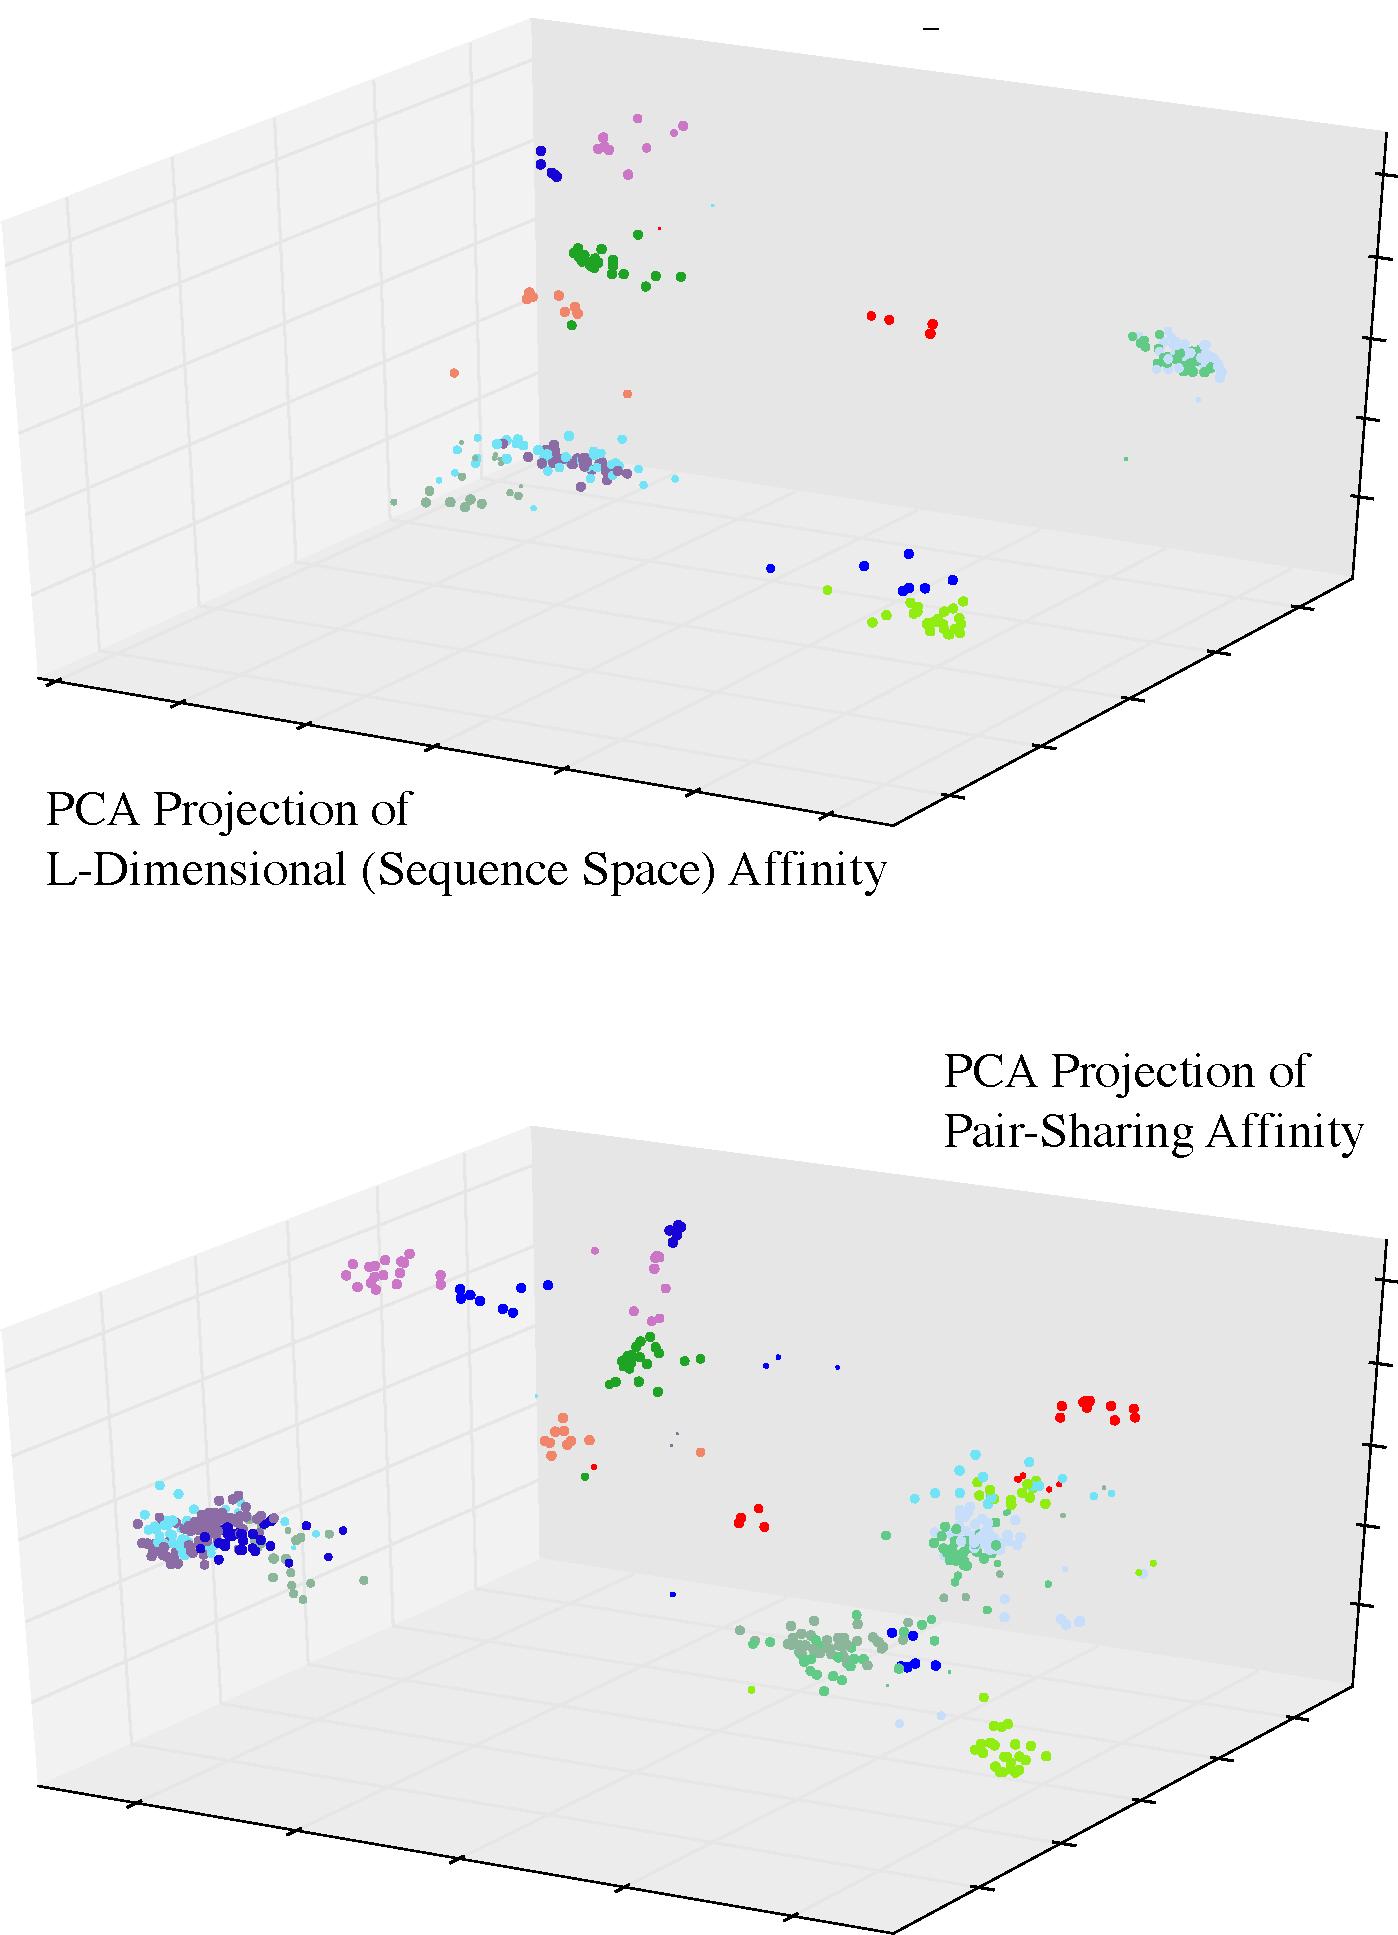
\includegraphics[width=2.3in]{figs/embeddings}
    \caption{Clusters derived from affinity propagation with pair sharing affinities. Top 3 PCA components of the correlation matrix for all structures are plotted for two different correlations. Top: $L$-dimensional correlation based on the projection described in \textbf{\ref{algebra}}. Bottom: Pair sharing correlation from \textbf{\ref{stochastic}}.}
    \label{fig:embeddings}
  \end{minipage}
  \hspace{0.5cm}
  \begin{minipage}[b]{0.45\linewidth}
    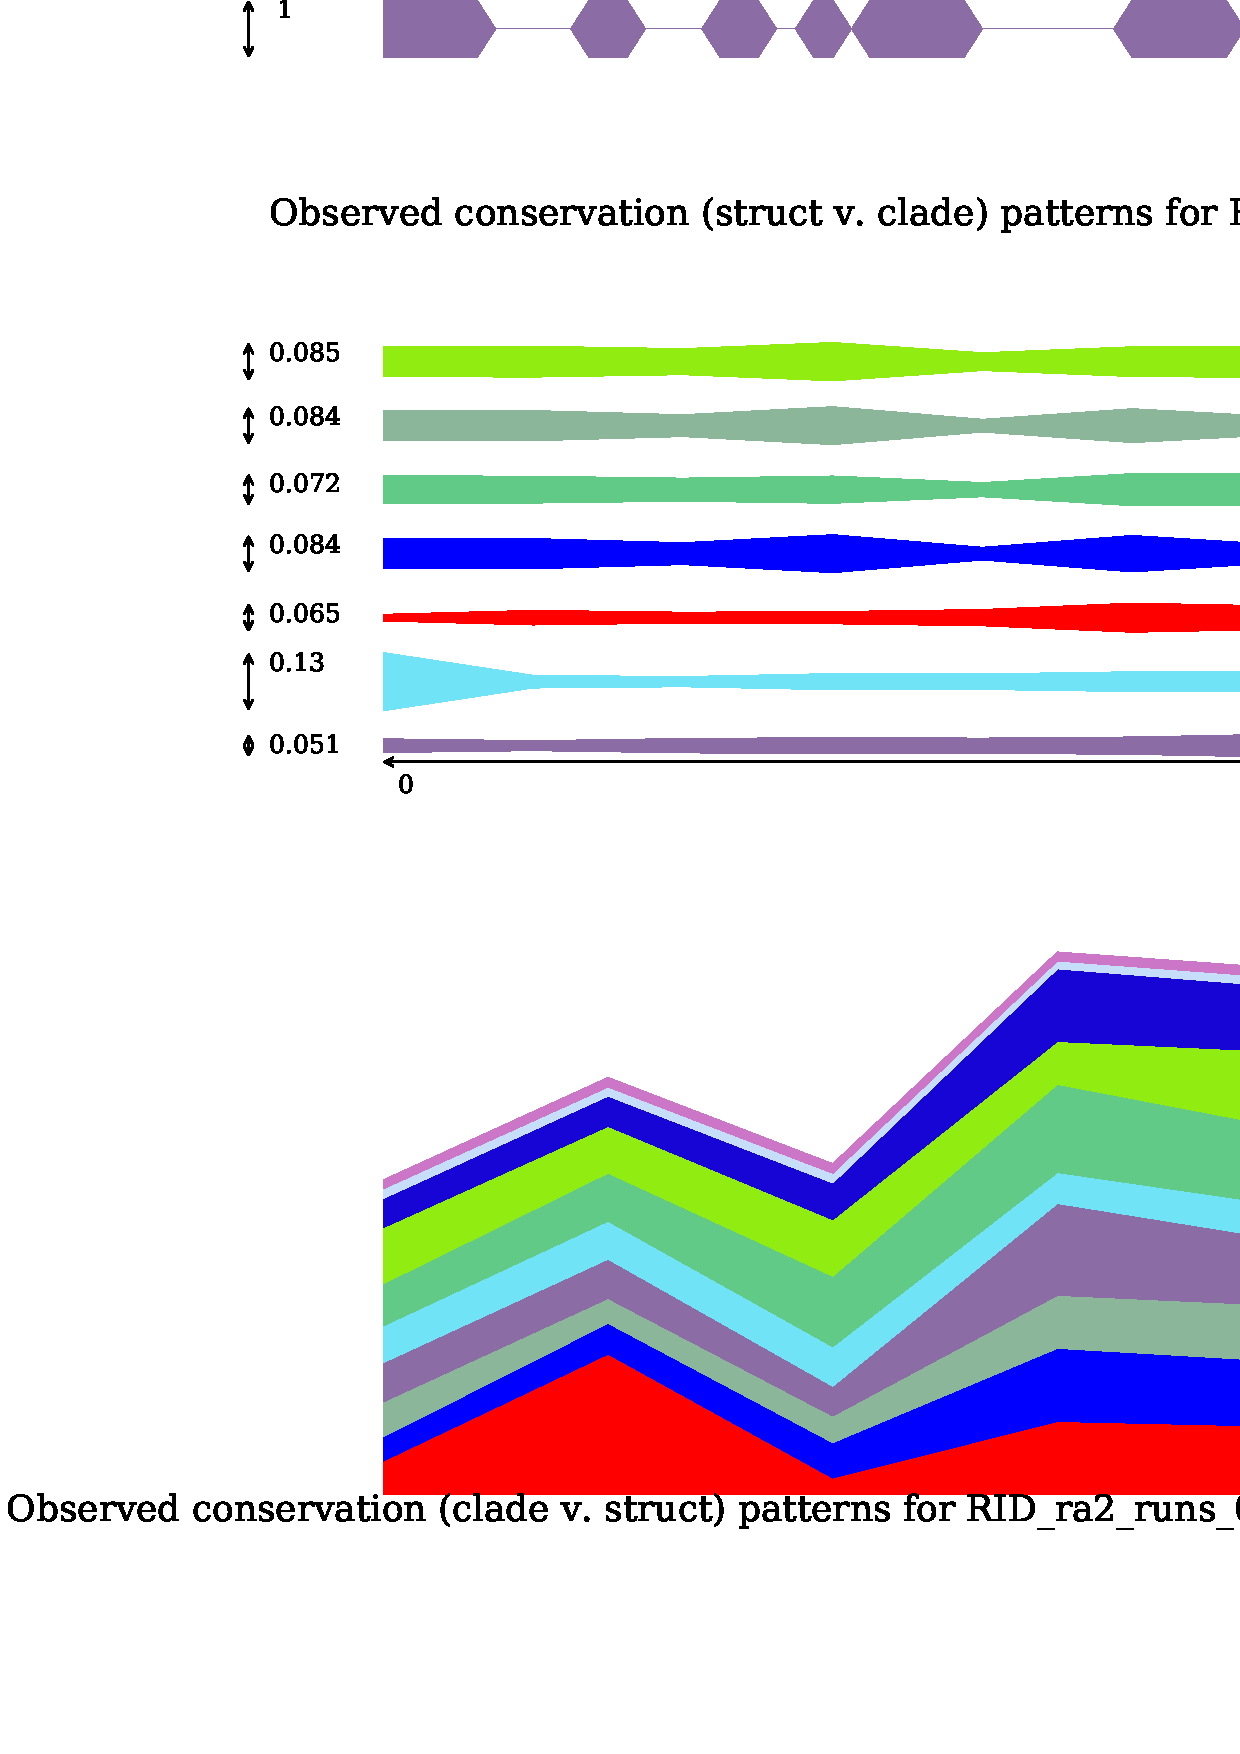
\includegraphics[width=3in]{figs/conservation}
    \centering
    \caption{Top: Expected conservation signatures $\theta^{S_i}_{\text{pred}}$ for foldings of RF00525, a CIS acting regulatory element playing a role in efficient translation of viral elements during host infection by the West Nile Virus. Middle: Conservation scores colored per structure $\{\mathcal{C}_i\}$ (x-axis is clade). Bottom: Conservation scores colored by per clade, (x-axis is structure).}
    \label{fig:conservation}
  \end{minipage}
  \centering

\end{figure}


\subsection{Stability Aware Prediction of Evolutionary Signatures}\label{prediction}
After establishing a set of candidate functional ncRNA functional structures, I computed expected conservation signals predicting the signature of evolution acting to preserve $S_i$: $\theta_{\text{pred}}(S_i)$. To lowest order, this signal would amount to observation of (1) exclusively base pair-preserving mutations at paired sites and (2) randomly distributed mutations at unpaired sites. In Fig. (\ref{fig:conservation}) such a binary signal is plotted for 7 folded states of a West Nile Virus Cis element whose folding alternates fall into two clear classes.

Noting however, that not all sites in the primary sequence and secondary structure of an ncRNA are equally important in determining folded conformation of ncRNA, I have implemented a more principled prediction for sequence/pairing conservation using an ``importance'' metric derived from the program RNAmutants\footnote{http://rnamutants.csail.mit.edu/}. Briefly, RNAmutants tests RNA structure stability over all possible $k$-fold mutations. To determine the importance of base-pairing of sequence elements $(i,j)$ in structure $S$, It was sufficient to compute the thermodynamic partition function of constrained folding to structure $S$ over all 2-fold mutations of bases $(i,j)$. 

Invoking an importance metric thus computed over all paired bases in $S$, it became possible to weight the evidence provided by pairing preserving (destroying) mutations in favor of (against) the hypothesis that natural selection acted to preserve paired components of the structure under consideration.\footnote{due to a bug in my RNAmutants wrapper that has persisted past submissiion time, reported results use the naive (binary) model for base-pair conservation importance}

\subsection{Phylogenetic  Deduction of Evolutionary Signatures}\label{deduction}
State of the art algorithms use a combination of thermodynamic modeling and phylogenetic analysis to deduce single predictions for optimal foldings of ncRNA families. One such algorithm is implemented by the program RNAalifold in the widely used Vienna RNA package. Augmenting a straightforward thermodynamic computation of structure for a familial consensus sequence, RNAalifold adds negative pseudo-energies to base positions where compensated mutations occur in the sequence alignment for a family. 

By counting compensated mutation observed in raw sequence alignments however, RNAalifold and similar programs fail to compute the true frequency of compensated mutation that would be observed in a parsimonious phylogenetic tree for a given ncRNA family. In this paper, I have attempted to remedy this by using PAML to infer maximum likelihood ancestor sequences in each subclade $\mathcal{C}_i$. Given perfect ancestor inference, such an approach would have the benefit both of providing twice the number of sequences per clade and providing a maximally parsimonious description of sequence variation for $\mathcal{Q}_i$ in terms pair-preserving and pair-disrupting mutations along phylogeny edges. Given such a count of mutational types implied by a tree for each pair in $S_i$, I construct a selection score over pairs from the relative frequencies of compensated and uncompensated mutants as well as the overall time spent paired and unpaired in the trees $\mathcal{T_C}$. In (\textbf{\ref{algebra}}) I denote this score ``$\text{Evo. Score}\left(P_{l,m} \right)^{\mathcal{C}_i}$''.

In practice, the inference ancestral nodes is imperfect both because the Rfam family is an incomplete set of leaf nodes for $\mathcal{C}_i$ and because the PAML substitution model assumes independence of sequence elements. Thus it was necessary to define a threshold at which to stop trusting ML nodes and revert to an alignment based metric for mutation description such as is implemented in RNAalifold. In fact, because this paper assumes a fixed set of reference structures it would be straightforward to implement an ML-ancestor inference algorithm that took into account dependencies between structurally specified base pairs and base pair stacks. No such approach is attempted here.\footnote{This paper \emph{does} however take advantage of the fixed set of structures under consideration in another important respect: realizing that the Rfam alignment for $\mathcal{F}$ is constructed with respect to a secondary structure covariance model derived from the single Rfam optimal structure $S_{opt}$, I compute sequence alignments of $\mathcal{Q_C}$ individually for computation of conservation strength for each $S_i \in \mathcal{S_F}$. In the final version of the algorithm, I will recompute trees for $\mathcal{C}_i$ in the same fashion.}


\subsection{Linear Algebraic Ranking of Suboptimals}\label{algebra}Having (\textbf{\ref{stochastic}}) computed candidate selected structures for $\mathcal{F}$ with  observed (\textbf{\ref{deduction}})  and predicted (\textbf{\ref{prediction}}) phylogenetic signatures of natural selection's action upon each, the final task of this paper is to discover a subset of candidate structures bearing responsibility for the evolutionary history of an ncRNA family.

To this end, several approaches could be envisioned. The simplest would be to simply rank structures in order of the ratio of compensated (base-pairing preserving) mutations to uncompensated mutations according seen in $\mathcal{F}$'s evolutionary history. Wishing instead to deduce a \emph{minimal} set of structures in a framework amenable to their comparison, I propose an alternative tack using $L_0$ regularized regression to describe observed signatures in terms of a minimal set of selected structures as follows:


\begin{description}
  \item[Splitting]  $\mathcal{F}$ into N clusters of similar sequences. These are the sets $\mathcal{Q}_i$ for clades $\mathcal{C}_i$.
    \item[Summing] evolutionary signals for each of $N$ clusters into vectors in $\mathbb{R}^L$
      \begin{equation*}
        \label{eq:sum}
        \theta_{\mathcal{C}_i} = \sum_{S_j\in|\mathcal{S}|}{\theta_{S_j}^{\mathcal{C}_i}}
      \end{equation*} 

      \begin{equation*} \theta_{S_j}^{\mathcal{C}_i}(l) = \left\{
          \begin{array}{rl} \text{Evo. Score}\left(P_{l,m} \right)^{\mathcal{C}_i}& \text{if } \exists m  \text{ s.t: paired}(l,m) \text{ in } S_j\\
            0 & \text{otherwise}\end{array} \right.
      \end{equation*} 

  where L is the length of the aligned sequence for the ncRNA family under consideration.\footnote{It is not intuitively clear that projection of structures (specified by $\mathcal{O}(L^2)$ pairs onto L length vectors) will be faithful and avoid excessive information loss. I pose the regression problem here in $L$-dim terms because by reducing the dimensionality of the prediction problem, I can increase the utility of the available data and decrease overfitting. In fact, one implication of Fig. (1) where clusters derived from pairwise affinities are scattered and remain coherent in PCA for pairwise ($L^2$-dim) and $L$-dim derived correlations is that the $L$-dim representation is somewhat faithful to full dimensional pairwise affinity. }
      \item[Regressing] with $L_0$ regularized least squares by treating the $N$ vectors $\theta_{\mathcal{C}_i}$ as $N$ observed points in $\mathbb{R}^L$ and $\theta_{\text{pred}}(S_i)$ from (\textbf{\ref{prediction}}) as an incomplete basis for $\mathbb{R}^L$. The structures with highest learned coefficients from regression will be considered the most likely to be under structural selection.
  \end{description}

\section{Future Directions}
Some preliminary results are plotted and analysis of selection on suboptimals in all Rfam families is under way. As an early control, I am running on 22 Rfam riboswitches (as a postive control where alternate structures are known to be functional) and tRNAs (a negative control where the opposite is true) and plan to present these results. Upcoming algorithmic improvements include a dependencey model for ancestor inference and principled incorporation of predicted signatures from RNAmutants.
\pagebreak{}
\renewcommand{\bibfont}{\small} 
\bibliographystyle{nature}
{\def\section*#1{}\bibliography{proposal}}
\end{document}
